\documentclass[a4paper,10pt]{article}
\usepackage[utf8x]{inputenc}
\usepackage{ismir2011,amsmath,cite}
\usepackage{graphicx}
%opening
\title{Large Scale Metric Learning For Music Similarity}
\author{Daniel \{Rosenberg, Erenrich\} }

\begin{document}
\maketitle

\begin{abstract}
Automatic music classification is an important problem in music analysis. In this paper, we use data from the ``Million Song Dataset'' to construct and evaluate music similarity metrics and metric learning techniques. While others have done metric learning on music datasets before, we evaluate which standard techniques perform best in both accuracy and time on this much larger dataset. We find that dramatically increasing the dataset size leads to larger performance gains than one might expect.
\end{abstract}

\section{Introduction}
Machine music analysis is a growing field in both industry and academia. One of the major difficulties with this work is that it requires large labeled corpuses which are difficult to obtain. The relatively new ``Million Song Dataset'' provides the music analysis community an opportunity to scale research to very large datasets with little organizational difficulty\cite{Bertin-Mahieux2011}. Already many papers of capitalized on this data to to solve such problems as playlist generation\cite{mcfee2011_nlp}, music classification and song cover-identification\cite{Bertin-Mahieux2011b}. 

Music similarity algorithms are especially useful because they can be used as subcomponents of algorithms like cover-identification and playlist generation. Previous work on music analysis was often performed on datasets as small as just 5000 songs\cite{Slaney_learninga}. It is now important that we reevaluate these techniques to determine how these algorithms scale in terms of accuracy and speed. It is not immediately obvious that all of our music metric-learning techniques will be able to scale. Others have already shown algorithmic techniques to speed up basic metrics of music similarity\cite{mcfee2011_sim}.

We performed metric learning across the ``Million Song Dataset'' in order to determine song similarity. Previous work has mainly relied upon definitions of similarity as songs appearing in the same album or being performed by the same artist. Other similarity measures have had poor performance. We take the creating artist as our ground truth for similarity.
\section{Data representation}
\subsection{Audio representation}
The ``Million Song Dataset'' provides features and metadata for a million songs as generated by the ``Echo Nest's'' music analysis software. This data includes such information as volume, length and beats per minute. In order to fit the entire dataset in memory and effectively work with it we projected down to a much smaller set of features. This set of features was strongly influenced by \cite{Slaney_learninga} though we chose to drop several features as they are not consistantly populated across the dataset. Less than one percent of the dataset appears to be invalid or improperly populated since some values are clearly incorrect. For example: songs which are listed as having zero beats were dropped from the analysis. 

We also added several features derived from the pitches contained in the songs. We chose to include the covariance matrix of pitches to get an idea of how pitches are grouped together. For instance, this should capture if a particular chord appears often. We also included the co-occurence counts so we can have a way to detect combinations that appear strongly correlated just because they occur infrequently. By adding quartiles of the max segment loudnesses, we hope to capture the song's progression over time. For instance, if a certain genre of songs tends to have a louder section towards the end, and another ends with a quiet repetition of the piece's theme, this feature will capture that.

\begin{itemize}
 \item Song length 
 \item Mean segment length - Echo Nest divides songs into segments of length less than a second
 \item Segment length variance
 \item Mean segment loudness
 \item Segment loudness variance
 \item Third quartile of max segment loudness - This gives us an idea of the distrubtion of loudness across segments
 \item First quartile of max segment loundess
 \item Mean segment begin loudness
 \item Segment begin loudness variance
 \item Beat interval variance
 \item Tatum confidence
 \item Mean tatum length
 \item Tatums per beat
 \item Time signature
 \item Time signature confidence
 \item Song mode
 \item Song mode confidence
 \item Pitch covariance matrix
 \item Pitch cooccurence counts
\end{itemize}

By eliminating all features that vary with time along the song the dimensionality of the data is reduced 308 numbers. This means that the 500GB dataset becomes just 1GB in size and so is much easier to analyze. Exactly how much information has been lost in the transformation is unclear. 
\subsection{Data labels}
We labeled our data with the song artist. Songs are considered to be similar if they share a common artist. We used this as our ground truth to judge our performance against.
\section{Algorithms}
\subsection{Whitening}
It has been shown throughout the literature that first whitening the dataset in order to ensure that the covariance matrix of the data is the identity matrix improves performance. We use KNN using euclidean distance and cosine similarity in conjunction with and without whitening. Evaluation of the distance metrics will be done by determining how well a KNN classifier is able to find songs that we have prelabeled as similar.

Note that for whitening we add in a small constant to all eigenvalues in order to diminish the impact of the smaller terms when we later take the inverse. This means that whitening here is only an approximation. 

Here we show our results on a compressed version of the dataset which only includes the top 500 most frequent artists and 25000 songs. A holdout test set of 5000 songs was used. This was done to decrease artist sparsity. A table of our accuracy is shown below.
\label{Foo} 
\begin{center}
\begin{tabular}{lllll}
KNN & Euclidean & Whitened & Cosine & Whitened\\
1 & 12.3\% & 19.3\% & 14.8\% & 20.3\%\\
3 & 12.1\% & 19.0\% & 14.5\% & 20.1\% \\
5 & 11.6\% & 18.2\% & 13.5\% & 19.4\% 
\end{tabular}
\end{center}
While these results are worse than what was presented in \cite{Slaney_learninga} which showed approximately 75\% accuracy for whitening we note that we are running over nearly 4 times more artists. Indeed considering the extreme differences between our datasets our results will never be directly comparable. Indeed whitening performs terribly on the full unrestricted dataset. This is to be expected as it is an entirely unsupervised technique.
\subsection{RCA Metric Learning}
Now we need to create a more sophisticated notion of distance than either euclidean or cosine similarity. Whitening is an unsupervised process and so is not taking advantage of all the information available to us. 

To get a more useful distance metric, we turned to the Mahalanobis metric. Under this metric, the distance between two vectors is: $d(x,y)=(x-y)'M(x-y)$, where M is a positive semidefinite matrix. An alternate definition uses $d(x,y)=||A(x-y)||_2$, where $M=A'A$. For instance, euclidean distance can be represented by $M=I$
We chose to learn a matrix $A$ that should improve our similarity metric using relevant component analysis.

Under RCA, we divide our data into 'chucklets', and essentially perform whitening seperately on each chunk. In the end, it weights more relevant features heavier than those that don't have as much of an effect.


% put description of that algorithm here

Our results over the full dataset are summarized in the following table.

\begin{center}
\begin{tabular}{ll}
Algorithm & Accuracy \\
Constant & 0.02\% \\
Euclidean & 0.2\% \\
Whitening & 0.52\% \\
RCA & 15.7\%
\end{tabular}
\end{center}
The constant algorithm which simply predicts the most common artist always is shown as a reference for comparison. RCA does more poorly here compared to the previous table because the number of artists has increased along with the dataset size itself. 

The main focus of this paper is the importance of dataset size. Its effect on test-accuracy is shown in the following plot.
\begin{center}
 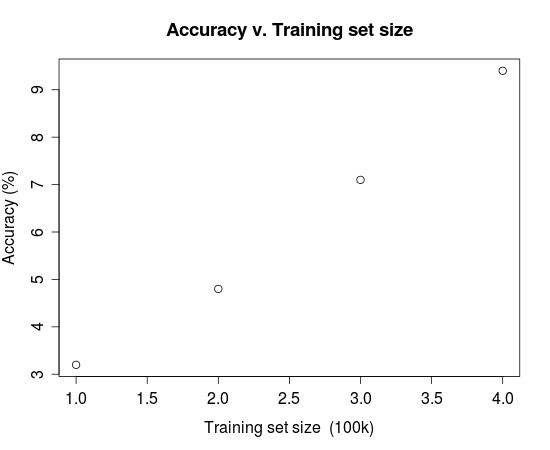
\includegraphics[scale=.4,keepaspectratio=true]{./training_set_v_accuracy.png}
 % training_set_v_accuracy.png: 550x450 pixel, 72dpi, 19.40x15.88 cm, bb=0 0 550 450
\end{center}

\subsection{Analysis}
The most striking result that we found was the large increase in performance with respect to dataset size. This was surprising because we would except a diminishing return with respect to the size of our dataset. Instead we found fairly robust gains as more data points were added. This suggests that an even larger dataset would provide even more impressive results. We though would sound a note of caution. Creating training and testing sets for this experiment is difficult. Randomly shuffling the dataset and extracting songs means that one might find that a particular artist lies only in the test set meaning that no algorithm could ever return the correct answer. 

There is also a problem in the reverse. Large testing datasets result in more classes (e.g. artists) to choose from which should increase error rates. To deal with that we might want to fix the number of classes we are dealing with and increase the number of examples per class. That is not an option with this particular dataset as it follows a long tailed distribution, and discarding artists with few songs would discard a large portion of the dataset.

\begin{center}
 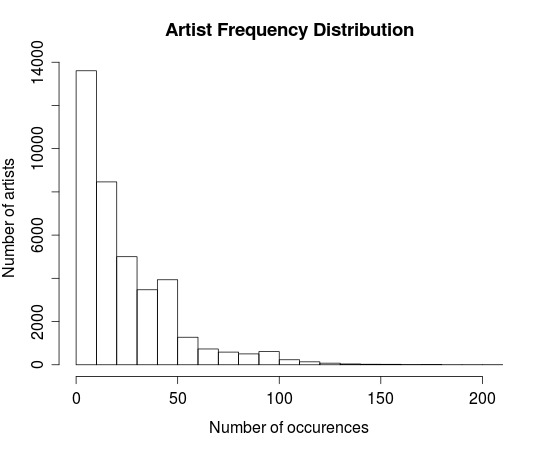
\includegraphics[scale=0.4,keepaspectratio=true]{./artist_frequency_dist.png}
 % artist_frequency_dist.png: 550x450 pixel, 72dpi, 19.40x15.88 cm, bb=0 0 550 450
\end{center}

The fact that KNN performance declines with the value of $k$, as seen in table \ref{Foo}, is also interesting. What we would really should be analyzing is the fraction of the time that the correct artist appears in the top $k$. Again this is because of the sparsity of the artist data. Settings $k$ to larger values means that we will never select artists which appear less frequently. Using a more dense indicator like genre should solve this problem as there are more exemplars per class.

\section{Conclusions and future work}
We conclude that future music ML research must be done on datasets of this size in order to generate relevant results. The increase in performance is simply too dramatic to ignore.

Metric learning for music is effective and seems to be a general solution to the problem of finding similar music and creating reccomendations based on sample songs. A disadvantage of the methods used in this paper is that we base similarity on the artist that created the work. A more effective system would be to use data from a reccomendation engine to perform metric learning. Songs which are often liked together (high listerner cooccurence) would then be deemed similar. This way we do not detect songs that sound the same but songs that are liked together which in the end is the main use case for algorithms of this type. 
\bibliography{refs}{}
\end{document}
